\documentclass[11pt,a4paper]{article}
\usepackage{fontspec}
\setmainfont{Times New Roman}
\usepackage[top=1.2cm,bottom=1.3cm,left=1.4cm,right=1.4cm]{geometry}
\usepackage{xcolor}
\usepackage{graphicx}
\usepackage{hyperref}
\usepackage{tabularx}
\usepackage{booktabs}
\usepackage{titlesec}
\usepackage{tcolorbox}
\tcbuselibrary{skins}
\usepackage{fancyhdr}
\usepackage{enumitem}
\usepackage{colortbl}
\usepackage{lastpage}
\usepackage{multicol}
\usepackage{array}
\usepackage{microtype}
\usepackage{amsmath}
\usepackage{tikz}
\usetikzlibrary{shapes.geometric, arrows.meta, positioning, calc}

% Modern Executive Monochrome Palette (Trắng Đen & Xám Chuẩn Doanh Nghiệp)
\definecolor{primary}{HTML}{000000}      % Pure Black
\definecolor{secondary}{HTML}{1A1A1A}    % Dark Charcoal
\definecolor{accent}{HTML}{000000}       % Pure Black (No green/blue)
\definecolor{accentlight}{HTML}{F3F4F6}  % Subtle Neutral Light Gray
\definecolor{softbg}{HTML}{F9FAFB}      % Crisp Off-White
\definecolor{hairline}{HTML}{D1D5DB}    % Neutral Border Gray
\definecolor{tagbg}{HTML}{F3F4F6}       % Neutral Light Box Gray
\definecolor{warnbg}{HTML}{F9FAFB}      % Neutral Background
\definecolor{warnborder}{HTML}{000000}  % Solid Black Frame
\definecolor{darktext}{HTML}{111111}    % Deep Black Text
\definecolor{mutedtext}{HTML}{4B5563}   % Charcoal Muted
\definecolor{tablealt}{HTML}{F9FAFB}    % Neutral Alternating Row

\hypersetup{
    colorlinks=true,
    linkcolor=primary,
    urlcolor=primary,
    citecolor=primary,
    pdfauthor={Le Tri Trung},
    pdftitle={Ho So Nang Luc va Bao Gia -- Team Ky Su Da Nang},
    pdfsubject={Phat trien Website SaaS Automation AI Integration},
    bookmarksdepth=2
}

% Header & Footer
\setlength{\headheight}{14pt}
\pagestyle{fancy}
\fancyhf{}
\rhead{\small\textcolor{mutedtext}{Hồ Sơ Năng Lực \& Báo Giá Kỹ Thuật --- Đội Ngũ Kỹ Sư Đà Nẵng}}
\lhead{\small\textbf{\textcolor{primary}{Lê Trí Trung \& Nhóm Cộng Sự}}}
\rfoot{\small\textcolor{mutedtext}{Trang \thepage/\pageref{LastPage}}}
\lfoot{\small\textcolor{mutedtext}{Tài liệu kỹ thuật \& Báo giá chính thức $\cdot$ letritrung.id.vn $\cdot$ \textit{Bảo mật}}}
\renewcommand{\headrulewidth}{0.4pt}
\renewcommand{\footrulewidth}{0.4pt}

% Clean Section Banner Macro
\newcommand{\sectionbanner}[2]{%
  \vspace{1.2mm}%
  \begin{tcolorbox}[colback=primary,colframe=primary,arc=1.5mm,boxrule=0pt,top=2mm,bottom=2mm,left=3mm,right=3mm]
    {\large\bfseries\color{white} #1 \quad$\vert$\quad \normalsize\color{white} #2}
  \end{tcolorbox}%
  \vspace{1.2mm}%
}

\tcbset{
    boxrule=0.7pt,
    arc=2mm,
    fonttitle=\bfseries,
    colback=white,
    colframe=hairline
}

\begin{document}

% ===============================================================
% TRANG 1: GIỚI THIỆU & ĐỘI NGŨ KỸ SƯ
% ===============================================================
\begin{tcolorbox}[colback=softbg,colframe=primary,arc=2.5mm,boxrule=1pt,top=2.5mm,bottom=2.5mm]
\begin{center}
    {\Large \textbf{\color{primary} HỒ SƠ NĂNG LỰC KỸ THUẬT \& BẢNG BÁO GIÁ DỰ ÁN}}\\[1.2mm]
    {\large \textbf{\color{primary} PHÁT TRIỂN WEBSITE KINH DOANH \& TỰ ĐỘNG HÓA SAAS --- AI AGENT}}\\[2mm]
    \small
    \textbf{Tech Lead:} Lê Trí Trung \quad$\cdot$\quad 
    \textbf{Hotline/Zalo:} 0782.399.721 \quad$\cdot$\quad 
    \textbf{Email:} letritrung2605@gmail.com\\[0.5mm]
    \url{https://letritrung.id.vn} $\cdot$ \url{https://biensovip.com} $\cdot$ \textbf{Trụ sở kỹ thuật:} Ngũ Hành Sơn, TP. Đà Nẵng
\end{center}
\end{tcolorbox}

\sectionbanner{PHẦN I}{GIỚI THIỆU ĐỘI NGŨ \& MÔ HÌNH LÀM VIỆC TRỰC TIẾP}

\begin{tcolorbox}[colback=tagbg,colframe=primary,arc=2mm,boxrule=0.8pt,top=1.8mm,bottom=1.8mm]
\small
\textbf{\color{primary} MÔ HÌNH KỸ SƯ 1-1 (NO MIDDLEMEN):} Khách hàng làm việc trực tiếp với Tech Lead. Xóa bỏ hoàn toàn chi phí trung gian agency (sales, account, quản lý đa cấp), tối ưu \textbf{30\%--40\% ngân sách} và rút ngắn thời gian bàn giao thực tế.
\end{tcolorbox}

\vspace{1mm}
\noindent Chúng tôi là nhóm \textbf{05 kỹ sư phần mềm chính quy} tại Đà Nẵng, chuyên sâu phát triển ứng dụng Web hiệu năng cao, sàn TMĐT, cổng thanh toán tự động VietQR và giải pháp AI Agent cho chủ shop bán lẻ, startup và doanh nghiệp vừa \& nhỏ (SMEs).

\vspace{1.2mm}
\noindent \textbf{\color{primary}\large 1. Đội Ngũ 05 Kỹ Sư Chuyên Trách (100\% Đại Học FPT --- Cựu FPT Software):}
\begin{itemize}[leftmargin=*,itemsep=2pt,topsep=1pt]
    \item \textbf{Lê Trí Trung --- Tech Lead \& Solutions Architect:} Quán quân Hackathon CV 2026, Top FPT ResFes. Cựu kỹ sư FPT Software. Trực tiếp kiến trúc sàn Biensovip.com, cổng VietQR $<0.5\text{s}$ và làm việc trực tiếp 1-1 với khách hàng.
    \item \textbf{Hà Văn Ân --- Kỹ sư Full-stack \& AI Integration:} Cựu kỹ sư FPT Software (Warehouse Inventory Systems). Tác giả nền tảng STEMGO (stemgo.net), đồng tác giả nghiên cứu ThreadLearn. Chuyên sâu Next.js App Router, Node.js, AI DeepSeek/Gemini \& RAG.
    \item \textbf{Nguyễn Thành Lộc --- Kỹ sư Backend .NET \& AI Pipeline:} GPA 3.5/4.0 ĐH FPT, cựu kỹ sư FPT Software Đà Nẵng. AI Team Lead BrandHub, Team Lead UniNest. Chứng chỉ Coursera AI Agent \& RAG LangChain. Chuyên sâu ASP.NET Core Web API \& FastAPI.
    \item \textbf{Nguyễn Minh Tuấn --- Kỹ sư Backend .NET \& Enterprise Systems:} Sở hữu chứng chỉ quốc tế \textbf{Microsoft Certified: Back-End Developer Professional} (2026). Cựu kỹ sư FPT Software, Team Lead VivuCar. Chuyên sâu .NET 8, SQL Server \& báo cáo quản trị.
    \item \textbf{Nguyễn Chơn Phước --- Kỹ sư Java Backend \& DevOps/Real-time:} Finalist InnoCodeCamp FPT. Cựu kỹ sư Acronic Solutions (Anti-DDoS Dashboard, Socket.IO real-time). Chuyên sâu Java Spring Boot, Docker, Linux/Nginx \& tối ưu tải duy trì Uptime 24/7.
\end{itemize}

\vspace{1.2mm}
\noindent \textbf{\color{primary}\large 2. Năng Lực \& Minh Chứng Kỹ Thuật Đã Khẳng Định:}
\begin{center}
\small
\renewcommand{\arraystretch}{1.1}
\begin{tabularx}{\textwidth}{>{\bfseries}p{5.5cm}X}
\toprule
\textbf{Thành Tích / Chứng Nhận} & \textbf{Chi Tiết Năng Lực Thực Chiến \& Đơn Vị Cấp} \\
\midrule
Microsoft Certified Professional & Chứng chỉ Quốc tế Microsoft Back-End Developer -- Microsoft (2026) \\
Quán quân Hackathon CV 2026 & Giải Nhất cuộc thi lập trình thực chiến công nghệ -- ĐH FPT Đà Nẵng (2026) \\
Cựu Kỹ Sư FPT Software & 4/5 thành viên đã qua thực tập và tham gia dự án thực tế tại FPT Software Đà Nẵng \\
Nghiên Cứu Khoa Học ResFes & Top 5 toàn quốc về mô hình AI phát hiện lỗi đa luồng, báo cáo tại ICTA 2026 \\
\bottomrule
\end{tabularx}
\end{center}

\vspace{1.2mm}
\noindent \textbf{\color{primary}\large 3. Cam Kết Quyền Lợi Khách Hàng:}
\begin{itemize}[leftmargin=*,itemsep=1.2pt,topsep=1pt]
    \item \textbf{Bàn giao 100\% mã nguồn (Source Code Ownership):} Khách hàng sở hữu toàn bộ bản quyền mã nguồn, cơ sở dữ liệu và tài liệu hướng dẫn vận hành, hoàn toàn không bị ràng buộc phụ thuộc.
    \item \textbf{Minh bạch tiến độ hằng ngày:} Cập nhật qua nhóm Zalo riêng, chạy thử nghiệm demo liên tục theo từng mốc.
\end{itemize}

\newpage

% ===============================================================
% TRANG 2: KIẾN TRÚC & TỰ ĐỘNG HÓA SAAS
% ===============================================================
\sectionbanner{PHẦN II}{KIẾN TRÚC KỸ THUẬT \& DÒNG CHẢY TỰ ĐỘNG HÓA SAAS}

\begin{tcolorbox}[colback=tagbg,colframe=primary,arc=2mm,boxrule=0.8pt,top=1.8mm,bottom=1.8mm]
\small
\textbf{\color{primary} VẬN HÀNH TỰ ĐỘNG KHÉP KÍN (CLOSED-LOOP AUTOMATION):} Website kinh doanh thế hệ mới là một cỗ máy bán hàng tự động 24/7. Cắt giảm 100\% khâu kiểm tra thủ công, tự động hóa từ bước tư vấn, tạo mã QR, khớp lệnh đến thông báo đơn hàng.
\end{tcolorbox}

\vspace{1mm}

% Elegant Vector Flow Diagram (Monochrome Black & White)
\begin{center}
\begin{tikzpicture}[
    node distance=0.45cm and 0.4cm,
    font=\small,
    box/.style={rectangle, rounded corners=2mm, draw=primary, fill=softbg, line width=0.8pt, minimum width=3.3cm, minimum height=1.6cm, align=center, inner sep=3pt},
    accentbox/.style={rectangle, rounded corners=2mm, draw=primary, fill=tagbg, line width=1.1pt, minimum width=3.3cm, minimum height=1.6cm, align=center, inner sep=3pt},
    arrow/.style={-{Stealth[scale=1.1]}, line width=1.2pt, color=primary}
]
    \node[box] (step1) {\textbf{\color{primary} 1. Khách Hàng}\\[1mm]\footnotesize Lướt web, chọn món\\\& ấn Đặt hàng nhanh};
    \node[accentbox, right=of step1] (step2) {\textbf{\color{primary} 2. VietQR Động}\\[1mm]\footnotesize Tự sinh mã QR đúng tiền\\\& mã đơn định danh};
    \node[accentbox, right=of step2] (step3) {\textbf{\color{primary} 3. Webhook Ngân Hàng}\\[1mm]\footnotesize Khớp lệnh tức thì $<0.5\text{s}$\\0đ phí duy trì};
    \node[box, right=of step3] (step4) {\textbf{\color{primary} 4. Tự Động Hóa}\\[1mm]\footnotesize Gạch nợ, báo Telegram\\AI CSKH tự động};

    \draw[arrow] (step1) -- (step2);
    \draw[arrow] (step2) -- (step3);
    \draw[arrow] (step3) -- (step4);
\end{tikzpicture}
\\[1mm]
{\footnotesize \textbf{Sơ đồ luồng xử lý:} Khách đặt hàng $\longrightarrow$ VietQR động $\longrightarrow$ Webhook ngân hàng tức thì $\longrightarrow$ Đồng bộ dữ liệu \& Báo cáo tự động}
\end{center}

\vspace{1.5mm}
\noindent \textbf{\color{primary}\large Bốn Trụ Cột Kỹ Thuật Đột Phá:}

\begin{enumerate}[leftmargin=*,itemsep=4pt,topsep=1pt]
    \item \textbf{Thanh Toán VietQR Tự Động \& Webhook Tức Thì ($<0.5$ giây):}
    \begin{itemize}[itemsep=1.5pt]
        \item Hệ thống tự tạo mã VietQR động chứa đúng số tiền và mã hóa đơn riêng biệt cho từng giao dịch.
        \item Ngay khi khách chuyển khoản, Webhook ngân hàng đẩy dữ liệu về máy chủ; hệ thống tự động gạch đơn và gửi thông báo qua Telegram/Zalo cho chủ cửa hàng trong vòng chưa đầy nửa giây.
        \item \textbf{Hiệu quả:} Hoàn toàn miễn phí duy trì (0đ phí cổng trung gian), không cần nhân viên trực soát bill.
    \end{itemize}

    \item \textbf{AI Agent DeepSeek --- Trợ Lý Bán Hàng \& Tư Vấn 24/7:}
    \begin{itemize}[itemsep=1.5pt]
        \item Tích hợp mô hình AI DeepSeek thông minh, chi phí API siêu tiết kiệm (chỉ \textbf{\$0.30--\$1.20/triệu token}, tiết kiệm hơn 90\% chi phí so với GPT-4/ChatGPT).
        \item Tự động học sâu danh mục sản phẩm, trả lời thắc mắc của khách hàng tự nhiên, gợi ý bán kèm (Cross-sell/Up-sell) và chốt đơn ngay trong khung chat.
    \end{itemize}

    \item \textbf{Tối Ưu Tốc Độ Google Core Web Vitals \& Chuẩn SEO Toàn Diện:}
    \begin{itemize}[itemsep=1.5pt]
        \item Đạt điểm hiệu năng Google Lighthouse \textbf{95--100/100}: LCP $\leq 2.5\text{s}$, INP $\leq 200\text{ms}$, CLS $\leq 0.1$.
        \item Định dạng ảnh tối ưu WebP/AVIF, Lazy Loading thông minh và kỹ thuật SSR Metadata giúp website luôn đạt thứ hạng cao trên trang nhất Google tìm kiếm.
    \end{itemize}

    \item \textbf{Quy Trình Vận Hành Tự Động Bằng n8n Workflow Engine:}
    \begin{itemize}[itemsep=1.5pt]
        \item Kết nối liền mạch toàn bộ công cụ quản lý: Google Sheets, CRM, Email tiếp thị và Zalo OA.
        \item Doanh nghiệp vận hành trơn tru, đồng bộ dữ liệu tức thì mà không cần mua phần mềm quản lý đắt đỏ.
    \end{itemize}
\end{enumerate}

\newpage

% ===============================================================
% TRANG 3: DỰ ÁN THỰC CHIẾN BIENSOVIP & 11 TÍNH NĂNG NỔI BẬT
% ===============================================================
\sectionbanner{PHẦN III}{MINH CHỨNG DỰ ÁN BIENSOVIP.COM \& 11 TÍNH NĂNG ĐỘT PHÁ}

\textit{``Sản phẩm thực tế khẳng định năng lực: Nền tảng giao dịch định danh trực tuyến đang vận hành hàng nghìn biển số mỗi ngày.''}

\vspace{1mm}
% Screenshots chính thức của Biensovip.com (Bao gồm Giao diện Sàn & Hệ thống Admin Portal Thực tế)
\begin{center}
    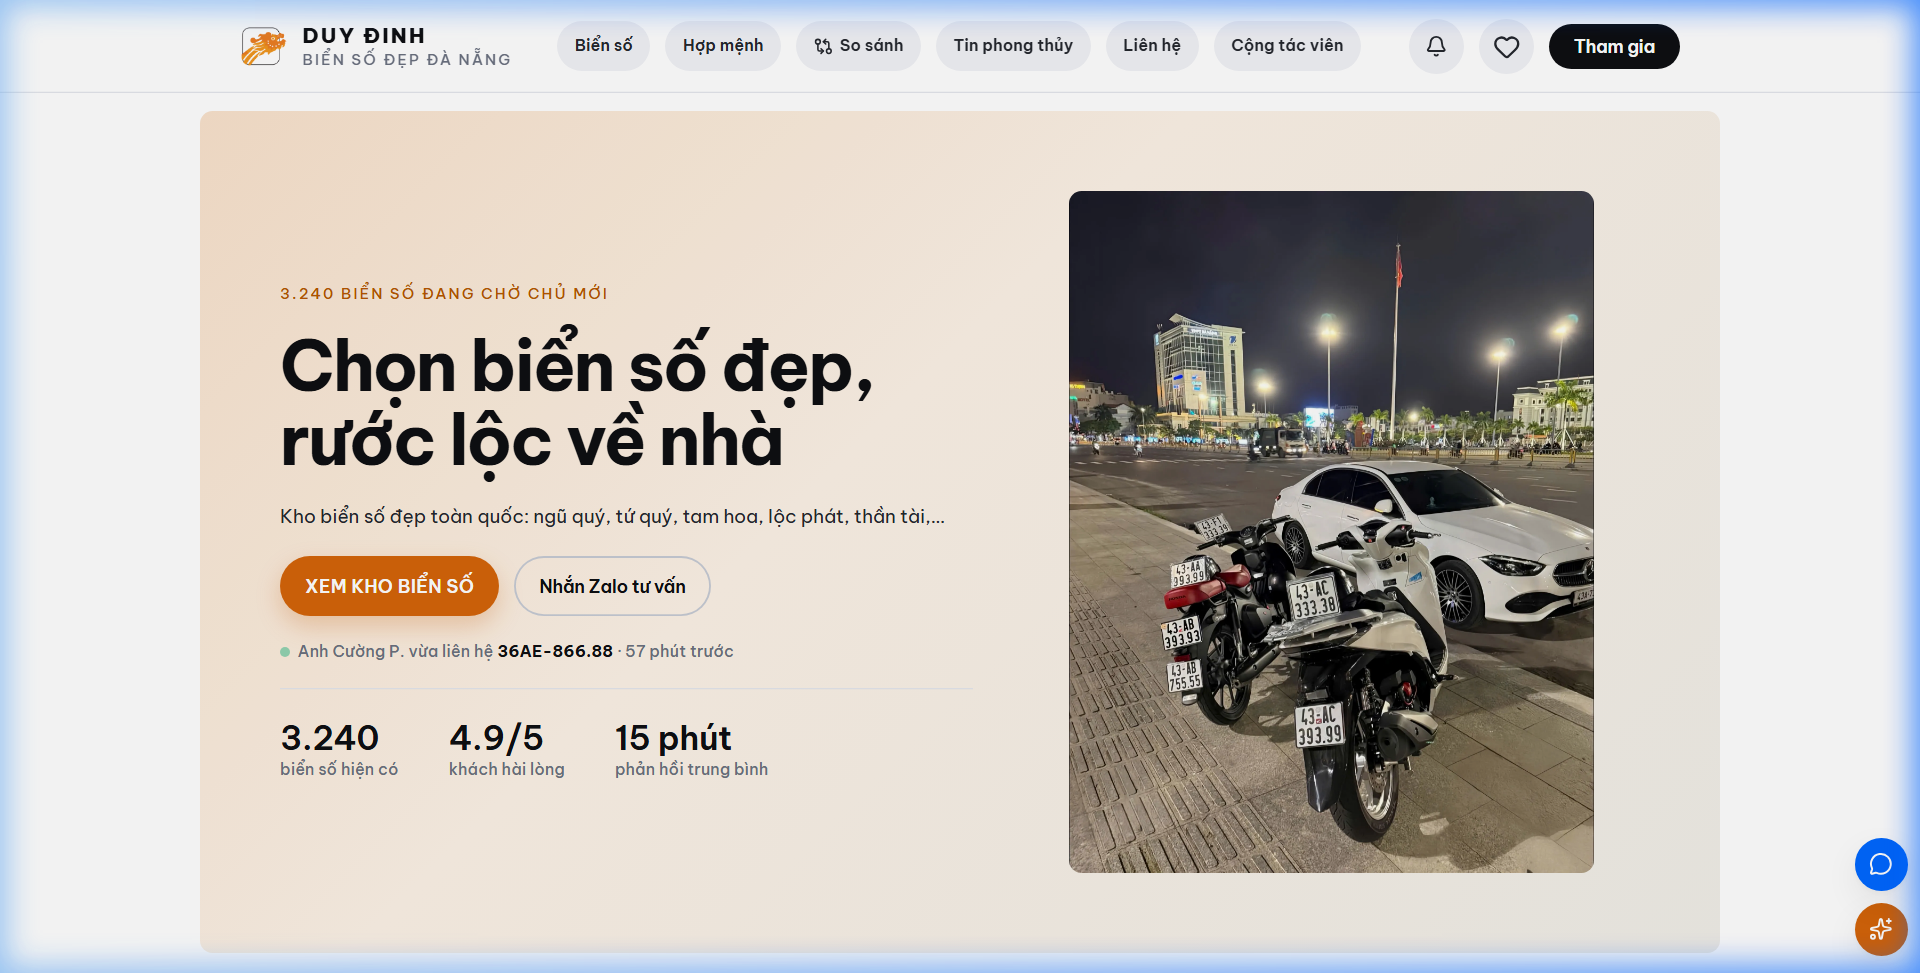
\includegraphics[width=0.98\textwidth,height=3.3cm,keepaspectratio]{images/biensovip_home_real.png}\\[0.5mm]
    {\footnotesize \textbf{Hình 1:} Giao diện sàn giao dịch Biensovip.com: Kho 3.240 biển số, lọc thế số tài lộc \& cổng cọc VietQR tự động}
\end{center}

\vspace{0.5mm}
\begin{center}
    \begin{minipage}[t]{0.49\textwidth}
        \centering
        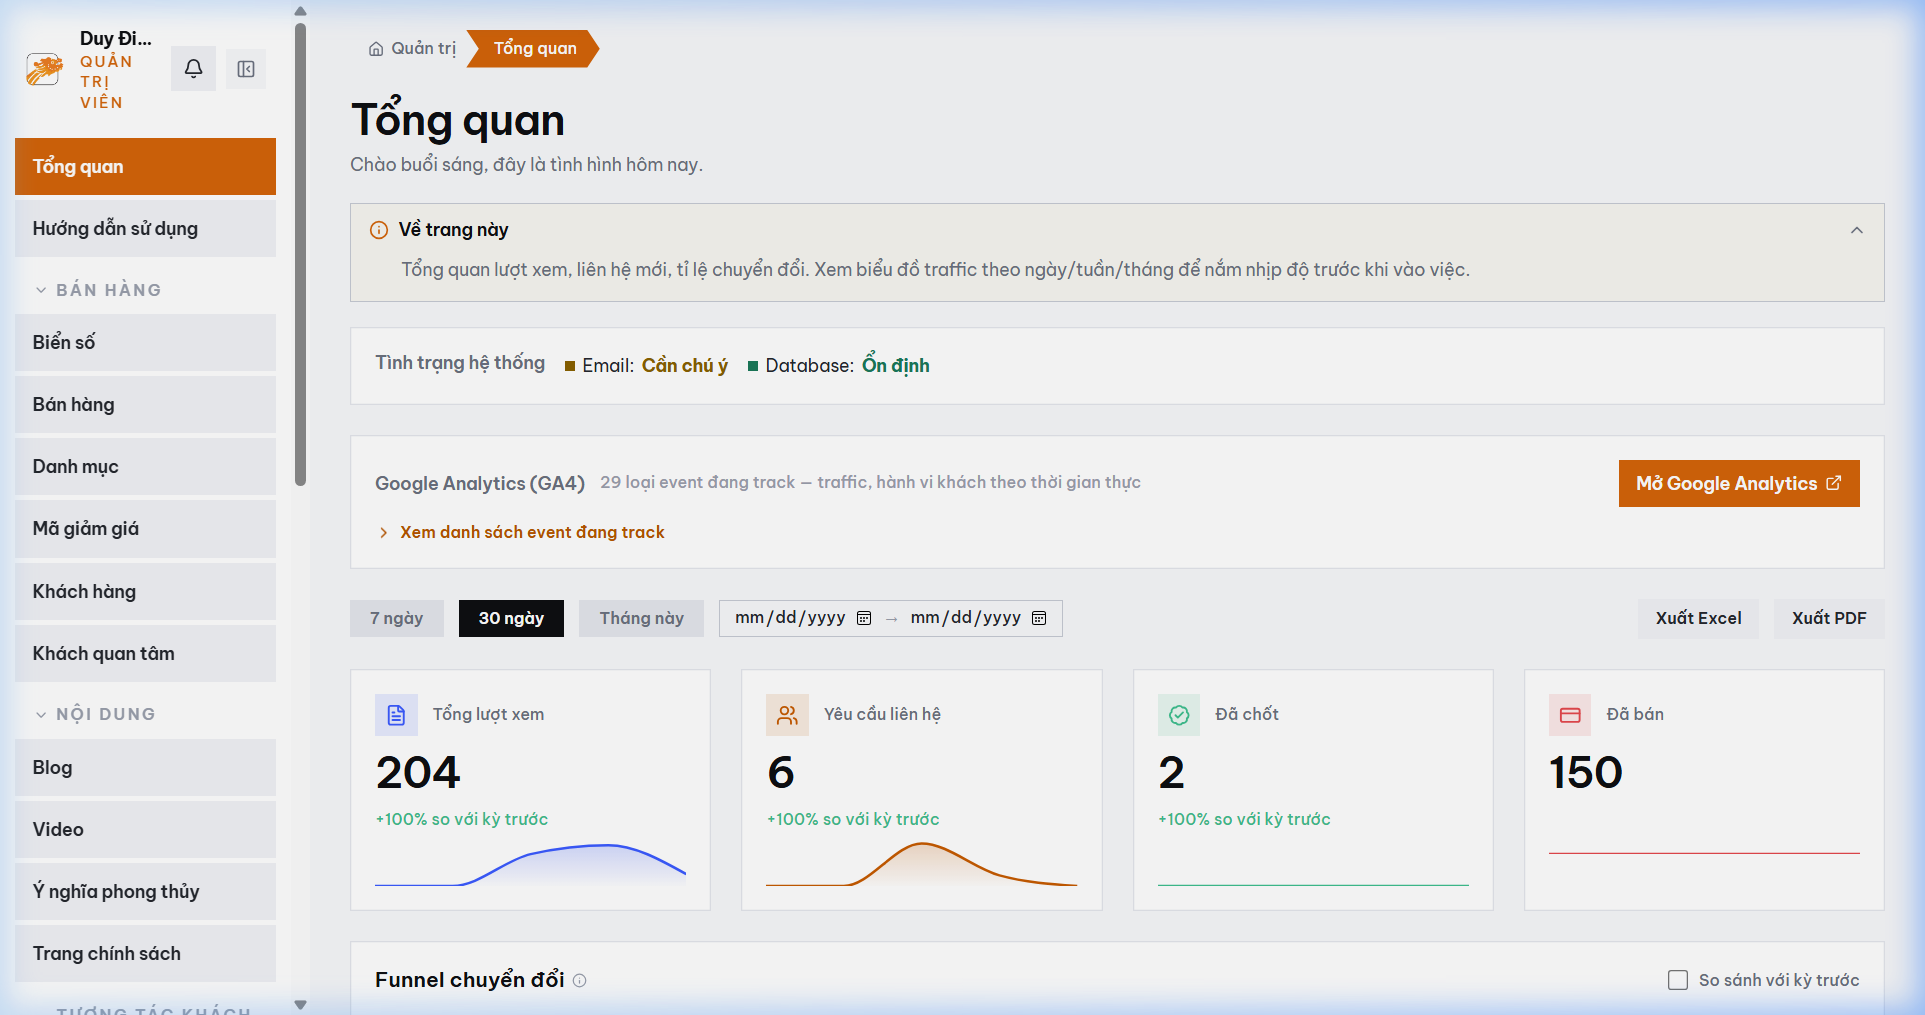
\includegraphics[width=\linewidth,height=2.8cm,keepaspectratio]{images/biensovip_admin_dashboard.png}\\[0.5mm]
        {\footnotesize \textbf{Hình 2a:} Admin Portal --- Dashboard Vận Hành: Doanh thu thực tế, phễu chuyển đổi, tracking GA4 \& xuất Excel/PDF}
    \end{minipage}
    \hfill
    \begin{minipage}[t]{0.49\textwidth}
        \centering
        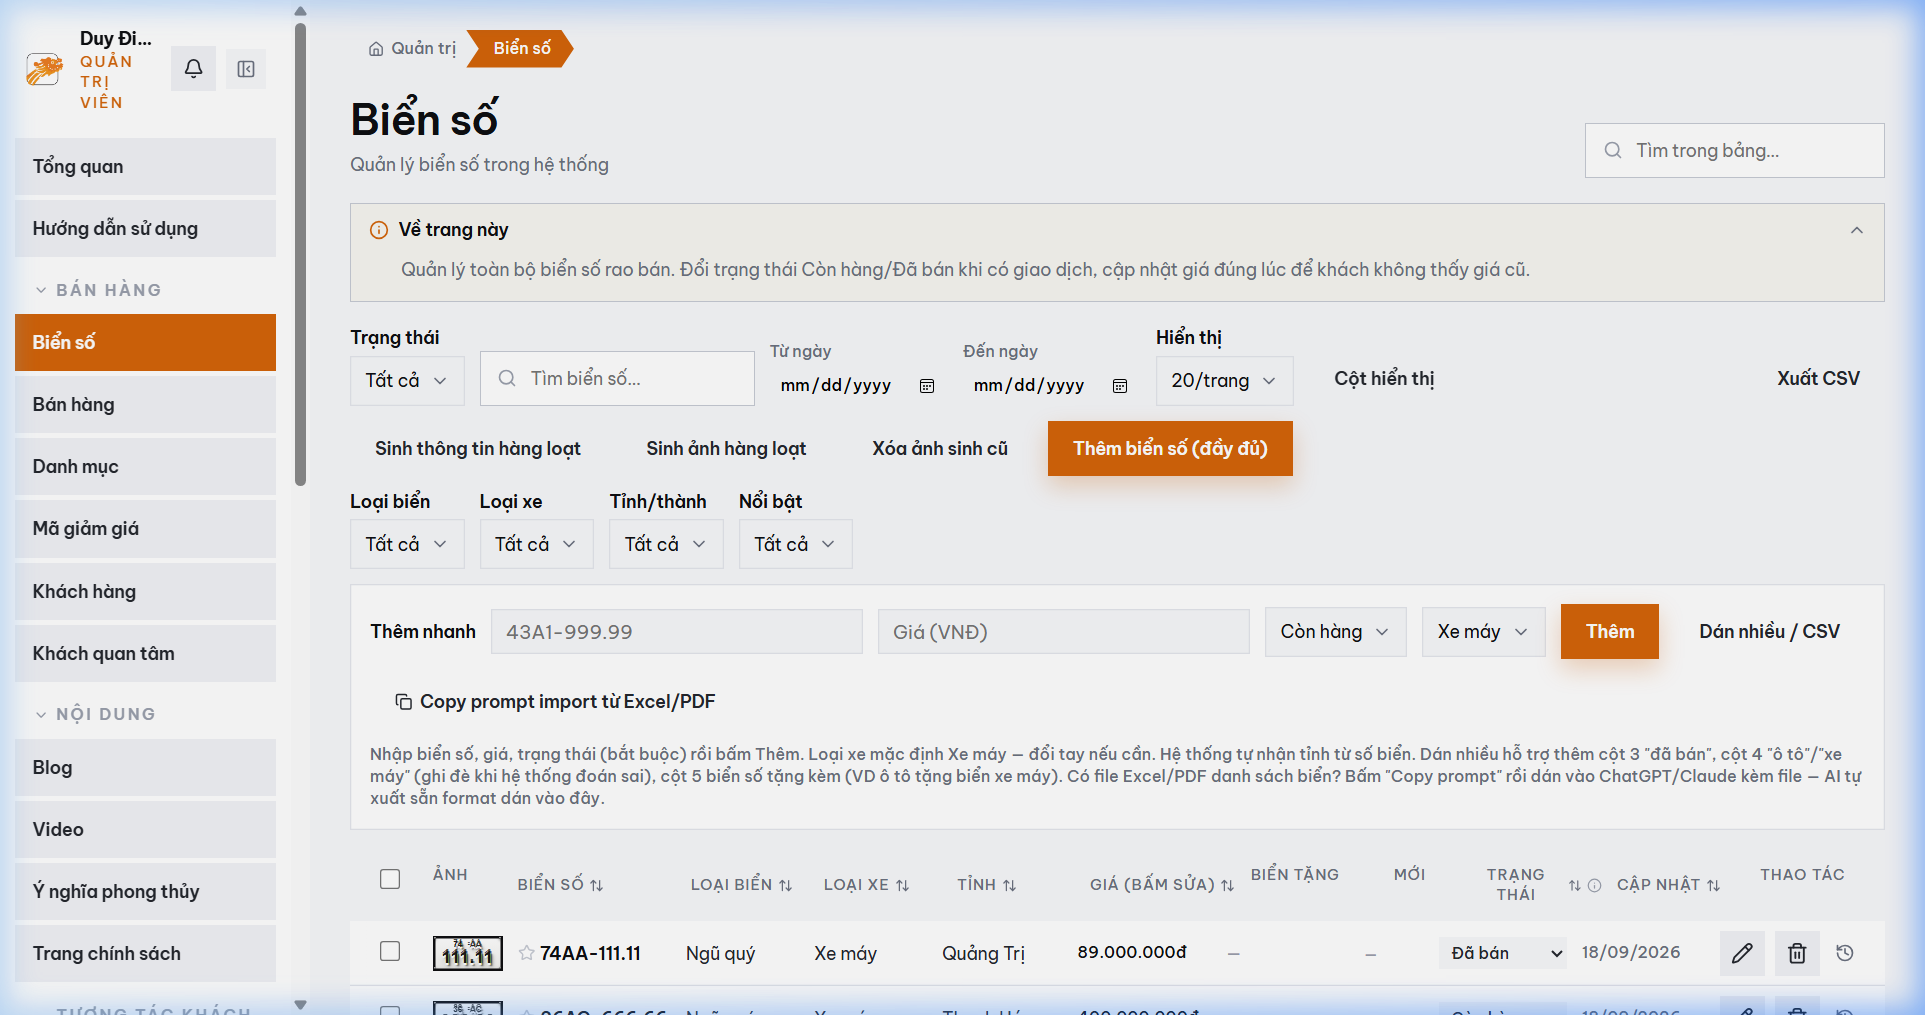
\includegraphics[width=\linewidth,height=2.8cm,keepaspectratio]{images/biensovip_admin_analytics.png}\\[0.5mm]
        {\footnotesize \textbf{Hình 2b:} Admin Portal --- Quản Lý Kho \& AI Generator: Kho 3.240 biển số, sinh prompt AI hàng loạt \& sửa giá inline}
    \end{minipage}
\end{center}

\vspace{1mm}
\begin{tcolorbox}[colback=softbg,colframe=primary,colbacktitle=primary,coltitle=white,arc=2mm,boxrule=0.8pt,top=1.5mm,bottom=1.5mm,title=\textbf{11 TÍNH NĂNG NỔI BẬT THU HÚT KHÁCH HÀNG TẠI BIENSOVIP.COM}]
\small
\begin{multicols}{2}
\begin{enumerate}[leftmargin=*,itemsep=1.2pt,topsep=0pt]
    \item \textbf{Tìm kiếm \& Lọc thông minh:} Tra cứu tức thì theo tỉnh thành, loại xe, thế số (Ngũ quý, Tứ quý, Tam hoa, Thần tài, Lộc phát 68/86...).
    \item \textbf{Mô phỏng 3D biển số kép:} Render trực quan cả 2 quy cách (Biển Dài \& Biển Ngắn) chuẩn kích thước thật.
    \item \textbf{Tra cứu biển hợp mệnh / Phong thủy:} Nhập ngày sinh $\rightarrow$ tự động giải mã Ngũ Hành \& gợi ý biển tương sinh.
    \item \textbf{So sánh biển số song song:} Đặt cạnh nhau tối đa 3 biển số so sánh giá bán, phong thủy, pháp lý giấy tờ.
    \item \textbf{Chốt biển \& Đặt cọc VietQR tức thì:} Tự sinh mã VietQR định danh, gạch đơn tức thì trong $<0.5\text{s}$.
    \item \textbf{Khóa bi quan (Pessimistic Lock):} Ngăn chặn triệt để 100\% nguy cơ bán trùng biển cho 2 khách cùng lúc.
    \item \textbf{Thông báo Social Proof real-time:} Popup thông báo khách vừa liên hệ/chốt biển tạo hiệu ứng đám đông.
    \item \textbf{Bộ đếm khách đang xem trực tiếp:} Hiển thị số người đang cùng xem biển kích thích tâm lý chốt đơn nhanh.
    \item \textbf{Trợ lý AI Chatbot 24/7 (DeepSeek):} Tư vấn biển hợp túi tiền \& hướng dẫn thủ tục cọc tự động.
    \item \textbf{Bộ sưu tập yêu thích (Wishlist):} Lưu biển theo dõi biến động giá \& nhận tin ưu đãi.
    \item \textbf{Cổng Cộng Tác Viên (Affiliate):} Quản lý mạng lưới bán hàng, phân chia hoa hồng tự động minh bạch.
\end{enumerate}
\end{multicols}
\end{tcolorbox}

\vspace{0.5mm}
\begin{tcolorbox}[colback=tagbg,colframe=primary,arc=2mm,boxrule=0.7pt,top=1mm,bottom=1mm]
\small
\textbf{CHỈ SỐ VẬN HÀNH THỰC TẾ:} \textbf{100+ Khách/ngày} (truy cập ổn định) $\cdot$ \textbf{$<$120ms Độ trễ API} (tối ưu SQL \& Redis) $\cdot$ \textbf{99.98\% Uptime} (Cloud Server 24/7) $\cdot$ \textbf{100\% VietQR tự động} (0đ phí duy trì cổng trung gian).
\end{tcolorbox}

\newpage

% ===============================================================
% TRANG 4: BÁO GIÁ 3 GÓI DỊCH VỤ CHUẨN XÁC VỚI THỰC TẾ
% ===============================================================
\sectionbanner{PHẦN IV}{BÁO GIÁ 3 GÓI DỊCH VỤ \& PHƯƠNG PHÁP ĐỊNH GIÁ}

\begin{tcolorbox}[colback=tagbg,colframe=primary,arc=2mm,boxrule=0.8pt,top=1.5mm,bottom=1.5mm]
\small
\textbf{\color{primary} NÓI KHÔNG VỚI CHI PHÍ ẨN --- ĐỊNH MỨC MAN-DAY MINH BẠCH:}\\
Mọi báo giá được bóc tách minh bạch dựa trên số lượng \textbf{Ngày Công Kỹ Thuật (Man-day / MD)} theo Tài liệu Đặc tả Yêu cầu (SRS). Cam kết tiến độ thực tế, chất lượng chỉn chu và không phát sinh phụ phí.\\[1mm]
\textbf{\color{primary} Đơn giá/MD tham chiếu:} Tech Lead: \textbf{1.8tr} $\cdot$ Backend: \textbf{1.5tr} $\cdot$ Frontend: \textbf{1.4tr} $\cdot$ AI/Automation: \textbf{1.4tr} $\cdot$ QA: \textbf{1.0tr} VNĐ
\end{tcolorbox}

\vspace{1mm}
\noindent \textbf{\color{primary}\large Bảng So Sánh 3 Gói Dịch Vụ Trọn Gói (Cập Nhật Chuẩn Xác Thực Tế):}\par\vspace{1.5mm}

\noindent
\begingroup
\small
\renewcommand{\arraystretch}{1.06}
\begin{tabularx}{\textwidth}{>{\raggedright\arraybackslash}p{2.6cm}Xccr}
\toprule
\textbf{Gói Dịch Vụ} & \textbf{Tính Năng Bàn Giao Chi Tiết} & \textbf{Nhân Lực} & \textbf{Tiến Độ} & \textbf{Giá Trọn Gói} \\
\midrule
\textbf{GÓI 1}\\MVP KHỞI NGHIỆP
& $\cdot$ Giao diện thiết kế theo yêu cầu, chuẩn Mobile First\newline
  $\cdot$ Danh mục sản phẩm/dịch vụ, trang chi tiết \& form liên hệ\newline
  $\cdot$ Nút gọi Hotline, chat Zalo \& Messenger nổi tiện lợi\newline
  $\cdot$ Chuẩn SEO Google cơ bản, chứng chỉ SSL miễn phí\newline
  $\cdot$ Cấu hình Hosting tối ưu + Bảo hành kỹ thuật \textbf{06 tháng}
& 1 Dev chính
& $\sim$\textbf{1.5 -- 2 tháng}
& \textbf{11.500.000₫} \\
\midrule
\rowcolor{accentlight}
\textbf{GÓI 2}\\MVP TỐC HÀNH\\{\color{primary}\textbf{\textit{Đề xuất $\cdot$ 2 Devs}}}
& $\cdot$ Toàn bộ tính năng của Gói Khởi Nghiệp\newline
  $\cdot$ \textbf{2 Kỹ sư code song song Frontend \& Backend}\newline
  $\cdot$ \textbf{Thanh toán VietQR tự động} sinh mã theo từng đơn hàng\newline
  $\cdot$ Quản lý đơn hàng, tự động báo qua \textbf{Telegram/Zalo Webhook}\newline
  $\cdot$ Cổng Admin CMS Panel quản trị sản phẩm, giá bán, duyệt đơn\newline
  $\cdot$ Miễn phí Cloud VPS trọn đời + Bảo hành \textbf{08 tháng}
& 2 Devs song song
& $\sim$\textbf{1.5 -- 2 tháng}
& \textbf{18.500.000₫} \\
\midrule
\textbf{GÓI 3}\\TOÀN DIỆN\\+ SAAS \& AI
& $\cdot$ Đầy đủ nền tảng Sàn TMĐT / Marketplace như Biensovip.com\newline
  $\cdot$ Đa phương thức: VietQR Webhook tự gạch nợ, VNPay, thẻ ATM\newline
  $\cdot$ \textbf{Tích hợp Trợ lý AI (DeepSeek API) 24/7} tư vấn chốt đơn\newline
  $\cdot$ \textbf{Admin Analytics chuyên sâu}: Biểu đồ doanh thu, tồn kho\newline
  $\cdot$ Tối ưu Core Web Vitals $<1\text{s}$ (Lighthouse 95--100/100)\newline
  $\cdot$ \textbf{Bàn giao 100\% Full Source Code} + Bảo hành \textbf{12 tháng} (24/7)
& Full team 5 người
& $\sim$\textbf{2 -- 2.5 tháng}
& \textbf{33.000.000₫} \\
\bottomrule
\end{tabularx}
\endgroup

\vspace{1.2mm}
\begin{tcolorbox}[colback=softbg,colframe=primary,colbacktitle=primary,coltitle=white,arc=2mm,boxrule=0.8pt,top=1.2mm,bottom=1.2mm,title=\textbf{CHÍNH SÁCH ĐÀM PHÁN NGÂN SÁCH \& TRỢ GIÁ KHỞI NGHIỆP}]
\small
\begin{itemize}[leftmargin=*,itemsep=1pt,topsep=0pt]
    \item \textbf{Trợ giá 20\%--30\%} cho cửa hàng mới mở, startup giai đoạn đầu hoặc đơn vị ký kết sớm trong tuần tư vấn.
    \item \textbf{Bóc tách linh hoạt theo ngân sách:} Có thể tinh giản module (AI Agent, VietQR) để giảm chi phí ban đầu và nâng cấp sau khi có dòng tiền ổn định.
    \item \textbf{Chia nhỏ thanh toán theo milestone:} Cơ chế 40\%/60\% đảm bảo sự an tâm tuyệt đối cho khách hàng.
\end{itemize}
\end{tcolorbox}

\newpage

% ===============================================================
% TRANG 5: QUY TRÌNH HỢP ĐỒNG & KÝ KẾT
% ===============================================================
\sectionbanner{PHẦN V}{QUY TRÌNH HỢP ĐỒNG, BẢO HÀNH \& KÝ KẾT}

\begin{enumerate}[leftmargin=*,itemsep=3.5pt,topsep=1pt]
    \item \textbf{Cơ Chế Giải Ngân An Toàn 40\% / 60\%:}
    \begin{itemize}[itemsep=1.5pt]
        \item \textit{Đợt 1 --- 40\% (Cọc kỹ thuật):} Thanh toán sau khi hai bên ký chốt Tài liệu Đặc tả Yêu cầu (SRS) và duyệt Wireframe giao diện.
        \item \textit{Đợt 2 --- 60\% (Nghiệm thu):} Chỉ thanh toán khi sản phẩm hoàn thiện 100\%, không còn lỗi nghiêm trọng (zero critical bug) và đã vận hành thử nghiệm trên tên miền chính thức trong ít nhất 48 giờ.
    \end{itemize}

    \item \textbf{Cam Kết Tiến Độ Thưởng / Phạt Rõ Ràng:}
    \begin{itemize}[itemsep=1.5pt]
        \item \textit{Phạt trễ hẹn:} \textbf{1\% giá trị hợp đồng / ngày trễ} (nếu do lỗi đội kỹ thuật), tối đa 10\%. Nếu trễ quá \textbf{15 ngày}: \textbf{hoàn trả 100\% tiền cọc ngay lập tức}.
        \item \textit{Thời gian ân hạn:} Tối đa 02 ngày làm việc cho trường hợp bất khả kháng được hai bên xác nhận.
    \end{itemize}

    \item \textbf{Chính Sách Hoán Đổi Tính Năng (Feature Change):}
    \begin{itemize}[itemsep=1.5pt]
        \item Cho phép hoán đổi miễn phí tối đa \textbf{20\% khối lượng tính năng} tương đương về độ phức tạp trong suốt quá trình phát triển dự án.
    \end{itemize}

    \item \textbf{Bảo Hành \& Hỗ Trợ Kỹ Thuật (SLA):}
    \begin{itemize}[itemsep=1.5pt]
        \item Bảo hành toàn diện \textbf{6--12 tháng}. Hỗ trợ xử lý sự cố khẩn cấp (P1) trong vòng \textbf{2 giờ}.
        \item Bàn giao trọn bộ mã nguồn, tài liệu API, sơ đồ cơ sở dữ liệu và video hướng dẫn quản trị chi tiết.
    \end{itemize}

    \item \textbf{Pháp Lý \& Nghĩa Vụ Thuế:}
    \begin{itemize}[itemsep=1.5pt]
        \item Đội ngũ tự chịu trách nhiệm kê khai và nộp thuế thu nhập cá nhân (TNCN) theo đúng luật định.
        \item Ký kết thỏa thuận bảo mật thông tin (NDA) và chuyển giao toàn bộ quyền sở hữu trí tuệ cho khách hàng.
    \end{itemize}
\end{enumerate}

\vspace{7mm}

\noindent
\begin{minipage}[t]{0.45\textwidth}
    \centering
    \textbf{\large ĐẠI DIỆN KHÁCH HÀNG / ĐỐI TÁC}\\[1mm]
    \textit{(Ký tên, ghi rõ họ tên \& đóng dấu nếu có)}\\[24mm]
    \rule{5.5cm}{0.4pt}\\[2mm]
    \small Ngày \rule{1cm}{0.4pt} / \rule{0.5cm}{0.4pt} / 2026
\end{minipage}
\hfill
\begin{minipage}[t]{0.45\textwidth}
    \centering
    \textbf{\large ĐẠI DIỆN ĐỘI NGŨ KỸ SƯ}\\
    \textit{Kiến trúc sư trưởng \& Trưởng nhóm Kỹ thuật}\\[20mm]
    \rule{5.5cm}{0.4pt}\\[2mm]
    \textbf{\large LÊ TRÍ TRUNG}\\
    \small Hotline/Zalo: 0782.399.721 $\cdot$ Đà Nẵng
\end{minipage}

\vspace{6mm}
\noindent\rule{\textwidth}{0.3pt}
\begin{center}
\footnotesize\textcolor{mutedtext}{\textbf{Nguồn dữ liệu \& Chuẩn công nghệ tham chiếu:}}
\end{center}
\begin{multicols}{2}
\footnotesize\textcolor{mutedtext}{
\begin{enumerate}[leftmargin=*,itemsep=0.5pt,label={[\arabic*]}]
    \item Ngân hàng Nhà nước VN: Báo cáo Thanh toán QR (2025).
    \item Google Web Vitals: Chuẩn LCP, INP, CLS (web.dev).
    \item n8n.io: Nền tảng tự động hóa hàng đầu thế giới (2026).
    \item DeepSeek API: AI Agent hiệu năng cao, tối ưu chi phí.
\end{enumerate}
}
\end{multicols}

\end{document}
